\documentclass[13pt,onlymath]{beamer}
\usefonttheme{serif}
\usepackage{graphicx,amsmath,amssymb,tikz,psfrag,epstopdf,fancyvrb}
\usepackage[lighttt]{lmodern}
%\usepackage{graphicx,psfrag}

\input defs.tex

%% formatting

\mode<presentation>
{
\usetheme{default}
}
\setbeamertemplate{navigation symbols}{}
\usecolortheme[rgb={0.13,0.28,0.59}]{structure}
\setbeamertemplate{itemize subitem}{--}
\setbeamertemplate{frametitle} {
    \begin{center}
      {\large\bf \insertframetitle}
    \end{center}
}

\newcommand\footlineon{
  \setbeamertemplate{footline} {
    \begin{beamercolorbox}[ht=2.5ex,dp=1.125ex,leftskip=.8cm,rightskip=.6cm]{structure}
      \footnotesize \insertsection
      \hfill
      {\insertframenumber}
    \end{beamercolorbox}
    \vskip 0.45cm
  }
}
\footlineon

\AtBeginSection[] 
{ 
    \begin{frame}<beamer> 
        \frametitle{Outline} 
        \tableofcontents[currentsection,currentsubsection] 
    \end{frame} 
} 

%% begin presentation

\title{\large \bfseries Combinatorial Games}

\author{Jaehyun Park\\[3ex]
CS 97SI\\
Stanford University}

\date{\today}

\begin{document}

\frame{
\thispagestyle{empty}
\titlepage
}

\begin{frame}{Combinatorial Games}
\BIT
\item Turn-based competitive multi-player games
\item Can be a simple win-or-lose game, or can involve points
\item Everyone has perfect information
\item Each turn, the player changes the current ``state'' using a valid ``move''
\item At some states, there are no valid moves
\BIT
\item The current player immediately loses at these states
\EIT
\EIT
\end{frame}


\section{Simple Games}

\begin{frame}{Combinatorial Game Example}
\BIT
\item Settings: There are $n$ stones in a pile. Two players take turns and remove 1 or 3 stones at a time. The one who takes the last stone wins. Find out the winner if both players play perfectly
\item State space: Each state can be represented by the number of remaining stones in the pile
\item Valid moves from state $x$: $x \rightarrow (x-1)$ or $x \rightarrow (x-3)$, as long as the resulting number is nonnegative
\item State 0 is the losing state
\EIT
\end{frame}

\begin{frame}{Example (continued)}
\BIT
\item No cycles in the state transitions
\BIT
\item Can solve the problem bottom-up (DP)
\EIT
\item A player wins if there is a way to force the opponent to lose
\BIT
\item Conversely, we lose if there is no such a way
\EIT
\item State $x$ is a winning state (W) if
\BIT
\item $(x-1)$ is a losing state,
\item OR $(x-3)$ is a losing state
\EIT
\item Otherwise, state $x$ is a losing state (L)
\EIT
\end{frame}

\begin{frame}{Example (continued)}
\BIT
\item DP table for small values of $n$:

\begin{center}
\begin{tabular}{|c|cccccccc|}
\hline
$n$&0&1&2&3&4&5&6&7 \\ \hline
W/L&L&W&L&W&L&W&L&W \\
\hline
\end{tabular}
\end{center}
\vfill
\item See a pattern?
\vfill
\item Let's prove our conjecture
\EIT
\end{frame}

\begin{frame}{Example (continued)}
\BIT
\item Conjecture: If $n$ is odd, the first player wins. If $n$ is even, the second player wins.
\vfill
\item Holds true for the base case $n=0$
\item In general,
\BIT
\item If $n$ is odd, we can remove one stone and give the opponent an even number of stones
\item If $n$ is even, no matter what we choose, we have to give an odd number of stones to the opponent
\EIT
\EIT
\end{frame}


\section{Minimax Algorithm}

\begin{frame}{More Complex Games}
\BIT
\item Settings: a competitive zero-sum two-player game
\item Zero-sum: if the first player's score is $x$, then the other player gets $-x$
\item Each player tries to maximize his/her own score
\item Both players play perfectly
\vfill
\item Can be solved using a \emph{minimax} algorithm
\EIT
\end{frame}

\begin{frame}{Minimax Algorithm}
\BIT
\item Recursive algorithm that decides the best move for the current player at a given state
\item Define $f(S)$ as the optimal score of the current player who starts at state $S$
\item Let $T_1, T_2, \ldots, T_m$ be states can be reached from $S$ using a single move
\item Let $T$ be the state that minimizes $f(T_i)$
\item Then, $f(S) = -f(T)$
\BIT
\item Intuition: minimizing the opponent's score maximizes my score
\EIT
\EIT
\end{frame}

\begin{frame}{Memoization}
\BIT
\item (Not \emph{memorization} but \emph{memoization})
\item A technique used to avoid repeated calculations in recursive functions
\item High-level idea: take a note (memo) of the return value of a function call. When the function is called with the same argument again, return the stored result
\item Each subproblem is solved at most once
\BIT
\item Some may not be solved at all!
\EIT
\EIT
\end{frame}

\begin{frame}[fragile]{Recursive Function without Memoization}
\begin{Verbatim}[xleftmargin=25pt]
int fib(int n)
{
    if(n <= 1) return n;
    return fib(n - 1) + fib(n - 2);
}
\end{Verbatim}
\vfill
\BIT
\item How many times is \verb,fib(1), called?
\EIT
\end{frame}

\begin{frame}[fragile]{Memoization using \texttt{std::map}}
\begin{Verbatim}[xleftmargin=25pt]
map<int, int> memo;
int fib(int n)
{
    if(memo.count(n)) return memo[n];
    if(n <= 1) return n;
    return memo[n] = fib(n - 1) + fib(n - 2);
}
\end{Verbatim}
\vfill
\BIT
\item How many times is \verb,fib(1), called?
\EIT
\end{frame}

\begin{frame}{Minimax Algorithm Pseudocode}
\BIT
\item Given state $S$, want to compute $f(S)$
\vfill
\item If we know $f(S)$ already, return it
\item Set return value $x \leftarrow -\infty$
\item For each valid next state $T$:
\BIT
\item Update return value $x \leftarrow \max\{x, -f(T)\}$
\EIT
\item Write a memo $f(S) = x$ and return $x$
\EIT
\end{frame}

\begin{frame}{Possible Extensions}
\BIT
\item The game is not zero-sum
\BIT
\item Each player wants to maximize his own score
\item Each player wants to maximize the difference between his score and the opponent's
\EIT
\item There are more than two players
\vfill
\item All of above can be solved using a similar idea
\EIT
\end{frame}


\section{Nim Game}

\begin{frame}{Nim Game}
\BIT
\item Settings: There are $n$ piles of stones. Two players take turns. Each player chooses a pile, and removes any number of stones from the pile. The one who takes the last stone wins. Find out the winner if both players play perfectly
\vfill
\item Can't really use DP if there are many piles, because the state space is huge
\EIT
\end{frame}

\begin{frame}{Nim Game Example}
\BIT
\item Starts with heaps of 3, 4, 5 stones
\BIT
\item We will call them heap A, heap B, and heap C
\EIT
\vfill
\item Alice takes 2 stones from A: $(1, 4, 5)$
\item Bob takes 4 from C: $(1, 4, 1)$
\item Alice takes 4 from B: $(1, 0, 1)$
\item Bob takes 1 from A: $(0, 0, 1)$
\item Alice takes 1 from C and wins: $(0, 0, 0)$
\EIT
\end{frame}

\begin{frame}{Solution to Nim}
\BIT
\item Given heaps of size $n_1, n_2, \ldots, n_m$
\item The first player wins if and only if the \emph{nim-sum} $n_1 \oplus n_2 \oplus \cdots \oplus n_m$ is nonzero ($\oplus$ is bitwise XOR operator)
\vfill
\item Why?
\BIT
\item If the nim-sum is zero, then whatever the current player does, the nim-sum of the next state is nonzero
\item If the nim-sum is nonzero, it is possible to force it to become zero (not obvious, but true)
\EIT
\EIT
\end{frame}


\section{Grundy Numbers (Nimbers)}

\begin{frame}{Playing Multiple Games at Once}
\BIT
\item Suppose that multiple games are played at the same time. At each turn, the player chooses a game and make a move. You lose if there is no possible move. We want to determine the winner
\EIT
\begin{center}
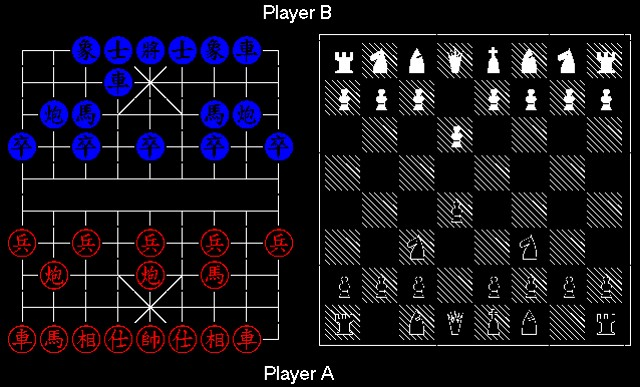
\includegraphics[height=0.5\textheight]{figures/games.jpg}

Figure from \url{http://sps.nus.edu.sg/~limchuwe/cgt/}
\end{center}
\end{frame}

\begin{frame}{Grundy Numbers (Nimbers)}
\BIT
\item For each game, we compute its \emph{Grundy number}
\item The first player wins if and only if the XOR of all the Grundy numbers is nonzero
\BIT
\item For example, the Grundy number of a one-pile version of the nim game is equal to the number of stones in the pile (we will see this again later)
\EIT
\vfill
\item Let's see how to compute the Grundy numbers for general games
\EIT
\end{frame}

\begin{frame}{Grundy Numbers}
\BIT
\item Let $S$ be a state, and $T_1, T_2, \ldots, T_m$ be states can be reached from $S$ using a single move
\vfill
\item The Grundy number $g(S)$ of $S$ is the smallest nonnegative integer that doesn't appear in $\{g(T_1), g(T_2), \ldots, g(T_m)\}$
\BIT
\item Note: the Grundy number of a losing state is 0
\item Note: I made up the notation $g(\cdot)$. Don't use it in other places
\EIT
\EIT
\end{frame}

\begin{frame}{Grundy Numbers Example}
\BIT
\item Consider a one-pile nim game
\item $g(0) = 0$, because it is a losing state
\item State 0 is the only state reachable from state 1, so $g(1)$ is the smallest nonnegative integer not appearing in $\{g(0)\} = \{0\}$. Thus, $g(1) = 1$
\item Similarly, $g(2) = 2$, $g(3) = 3$, and so on
\item Grundy numbers for this game is then $g(n) = n$
\BIT
\item That's how we got the nim-sum solution
\EIT
\EIT
\end{frame}

\begin{frame}{Another Example}
\BIT
\item Let's consider a variant of the game we considered before; only 1 or 2 stones can be removed at each turn
\item Now we're going to play many copies of this game at the same time
\item Grundy number table:

\begin{center}
\begin{tabular}{|c|cccccccc|}
\hline
$n$&0&1&2&3&4&5&6&7 \\ \hline
$g(n)$&0&1&2&0&1&2&0&1 \\
\hline
\end{tabular}
\end{center}
\EIT
\end{frame}

\begin{frame}{Another Example (continued)}
\BIT
\item Grundy number table:

\begin{center}
\begin{tabular}{|c|cccccccc|}
\hline
$n$&0&1&2&3&4&5&6&7 \\ \hline
$g(n)$&0&1&2&0&1&2&0&1 \\
\hline
\end{tabular}
\end{center}
\vfill
\item Who wins if there are three piles of stones $(2, 4, 5)$?
\item What if we start with $(5, 11, 13, 16)$?
\item What if we start with $(10^{100}, 10^{200})$?
\EIT
\end{frame}

\begin{frame}{Tips for Solving Game Problems}
\BIT
\item If the state space is small, use memoization
\item If not, print out the result of the game for small test data and look for a pattern
\BIT
\item This actually works really well!
\EIT
\item Try to convert the game into some nim-variant
\item If multiple games are played at once, use Grundy numbers
\EIT
\end{frame}

\end{document}
